
\phantomsection

\chapter{Contexto}%\label{cap:Contexto}

O presente capítulo apresenta o contexto no qual o dispositivo desenvolvido pode ser aplicado mostrando os conceitos de dinâmica veicular longitudinal, principais sistemas de segurança envolvidos, e os esforços mecânicos presentes nos componentes de interesse.

\section{Dinâmica veicular}

%DESCREVER UM EIXO DE TRANSMISSAO

Dinâmica veicular é o campo da física aplicada que investiga o comportamento de um veículo automotor em condições de uso e estáticas, a norma SAE J670 (2008) adota o sistema de coordenadas ilustrado na \autoref{fig:Fig_301} para um veículo genérico com a origem na posição do seu centro de massa nas análises dinâmicas em veículos terrestres.

\begin{figure}[htb]
	\caption{\label{fig:Fig_301}Sistema de coordenadas SAE}
	\begin{center}
		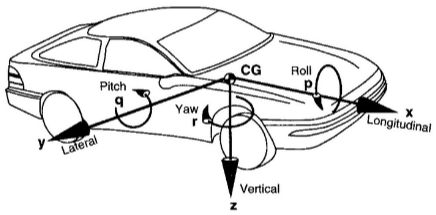
\includegraphics[width=\textwidth]{images/img301.jpg}
	\end{center}
	\fonte{**Tsirogiannis (2015)**}
\end{figure}	

A dinâmica veicular é composta por três campos de estudo (longitudinal, lateral e vertical) que investigam o comportamento do veículo ao longo das direções padrões. A dinâmica longitudinal veicular engloba a análise da movimentação do veículo no seu eixo de pitch e na direção longitudinal causadas pelo trem de força, conjunto de componentes responsáveis pela geração de potencia e transmissão do movimento para os pneus do eixo de tração, e do sistema de frenagem. A \autoref{fig:Fig_302} ilustra os principais componentes presentes no trem de força em um veículo com tração traseira.

\begin{figure}[htb]
	\caption{\label{fig:Fig_302}Elementos principais do trem de potência}
	\begin{center}
		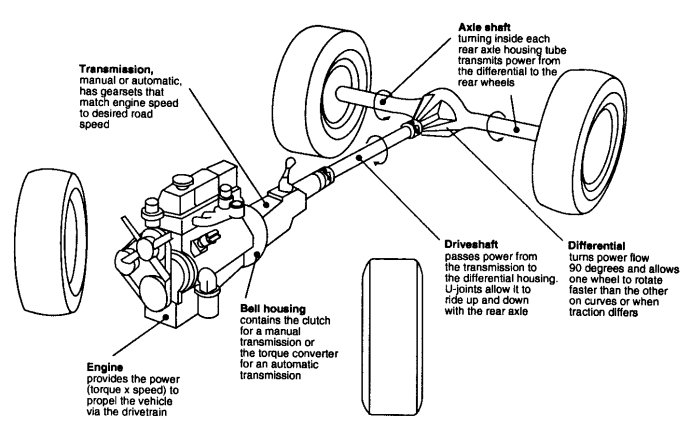
\includegraphics[width=\textwidth]{images/img302.jpg}
	\end{center}
	\fonte{**Gillespie (1992)**}
\end{figure}

Nas análises simplificadas de dinâmica veicular a unidade motora é modelada por suas curvas de torque e potência, os componentes da transmissão como as respectivas relações de amplificação de torque e as rodas pelo seu raio e coeficiente de atrito do contato entre pneu e pista. A figura 3 mostra o diagrama de corpo livre de um automóvel simplificado. Em um veículo com tração unicamente traseira e sem a presença de reboque, as forças de tração geradas nas interfaces pneu pista frontais e reações das cargas traseiras não estarão presentes, simplificando a análise.

\begin{figure}[htb]	
	\caption{\label{fig:Fig_303}Principais forças envolvidas na dinâmica longitudinal}
	\begin{center}
		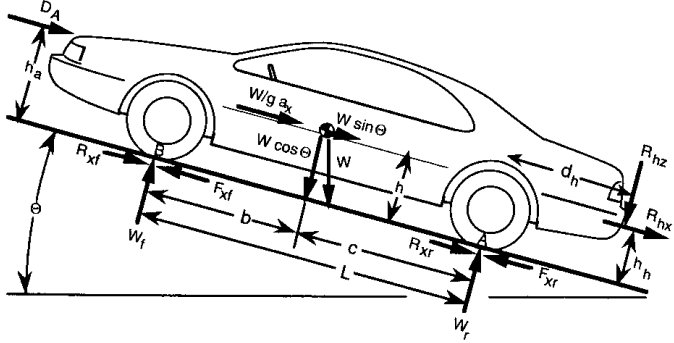
\includegraphics[width=\textwidth]{images/img303.jpg}
	\end{center}
	\fonte{**Gillespie (1992)**}
\end{figure}

\subsection{Capacidade de aceleração}

Dentre as análises do veículo na dinâmica longitudinal pode-se definir sua capacidade máxima de aceleração, Gillespie (1992) afirma que esse potencial é determinado por um entre dois limites, definidos primariamente pela velocidade do veículo, em altas velocidades espera-se o limite seja relacionado a potência da unidade motora, e em baixas velocidades a capacidade de tração das rodas motrizes.

Presumindo que haja potência suficiente na unidade motora, a aceleração será limitada pelo coeficiente de atrito na interface entre o pneu das rodas motrizes e a superfície de contato nesse caso, o limite de tração é mostrado pela \autoref{eq:Eq_301}.

O coeficiente de atrito do contato pneu pista é dependente de diversos fatores, entre eles a área de superfície de contato do pneu, tipo de compósito e condição, parâmetros operacionais como temperatura e pressão, carga aplicada no pneu, etc.

\vspace{\baselineskip}

\begin{equation}\label{eq:Eq_301}
F_{x} = \mu W
\end{equation}

sendo

$F_{x}$: Força de tração gerada pelos pneus

$\mu$: Coeficiente de atrito máximo do contato

W: Carga aplicada no eixo de tração

\vspace{\baselineskip}

\section{Esforços em componentes}


Os sistemas veiculares responsáveis pela transmissão do torque no trem de potencia, uma vez que são compostos de elementos rotativos, apresentam tensões geradas pelas cargas de torque e flexão durante a operação.

%Esse capítulo ilustra o desenvolvimento matemático a ser utilizado nas etapas de análises computacionais e validação do conceito experimental.

%\subsection{Deformação de viga devido a carga estática}
%
%Em uma viga retangular engastada, a tensão máxima causada por flexão é dada pela \autoref{eq:Eq_501}.
%
%\begin{equation}\label{eq:Eq_501}
%\sigma = \frac{My}{I}
%\end{equation}
%
%onde
%
%$\sigma$: Tensão causada pelo momento fletor
%
%M: Momento fletor na posição x
%
%y: Distância entre superfície de análise e linha neutra
%
%I: Segundo momento de inércia da seção transversal
%
%\vspace{\baselineskip}
%
%O segundo momento de inércia de uma seção retangular em relação ao seu centro é dado pela \autoref{eq:Eq_502}.
%
%\begin{equation}\label{eq:Eq_502}
%I = \frac{bh^{3}}{12}
%\end{equation}
%
%onde
%
%b: Largura da seção retangular
%
%h: Altura da seção retangular
%
%\vspace{\baselineskip}
%
%Os valores de deformação para um caso geral podem ser facilmente obtido utilizando a lei de Hooke representado pela \autoref{eq:Eq_503}.
%
%\begin{equation}\label{eq:Eq_503}
%\sigma = E \varepsilon
%\end{equation}
%
%onde
%
%E: Módulo de elasticidade do material
%
%$\varepsilon$: Deformação
%
%\vspace{\baselineskip}
%
%Então, pode-se encontrar uma equação geral para a deformação de uma viga genérica sujeita a um momento M \autoref{eq:Eq_504}.
%
%\begin{equation}\label{eq:Eq_504}
%\varepsilon = \frac{6My}{Ebh^{2}}
%\end{equation}
%
%\vspace{\baselineskip}

\subsection{Deformação de um eixo em torção}

Norton (2013) afirma que quando barras estão solicitadas por um momento em relação ao seu eixo longitudinal, diz-se que estão sob torção, esse tipo de momento aplicado é denominado torque e está situação é comum em eixos que transmitem potência. A \autoref{fig:Fig_501} ilustra os ângulos de deformação vistos em um eixo e a distribuição de tensão de cisalhamento ao longo da sua seção transversal, os valores são dados pela \autoref{eq:Eq_505} e \autoref{eq:Eq_506},


\begin{figure}[htb]
	\caption{\label{fig:Fig_501}Deflexão e distribuição de tensão devido a torção}
	\begin{center}
		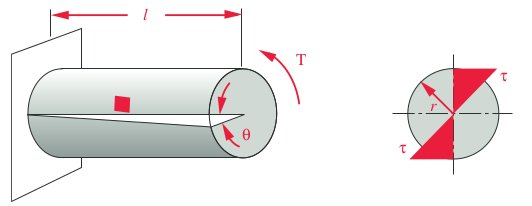
\includegraphics[width=\textwidth]{images/img501.jpg}
	\end{center}
	\fonte{**Norton 4ed**}
\end{figure}

\begin{equation}\label{eq:Eq_505}
\theta = \frac{Tl}{GJ}
\end{equation}

\begin{equation}\label{eq:Eq_506}
\tau = \frac{Tr}{J}
\end{equation}

onde:

$\theta$: ângulo de torção

$\tau$: tensão superficial causada pela torção

$T$: valor de torque aplicado

$r$: raio do eixo

$l$: comprimento até o ponto de análise

$G$: Modulo de cisalhamento do material

$J$: Momento de inércia polar da seção transversal

\vspace{\baselineskip}

As equações consideram a operação do componente apenas em regime de deformação elástico, logo os valores esperados de $\theta$ serão relativamente pequenos. (escrever sobre a influencia disso na operação do eixo)

\vspace{\baselineskip}

\section{Sensoriamento de deformações}

Com o objetivo de obter grandezas associadas em um veículo durante sua operação, são utilizado sensores baseados na sua variação de resistência.

\subsection{Extensômetro}

Extensômetros são sensores que sofrem alterações de resistência elétrica conforme a deformação ocorrida na superfície em que são aplicados, uma relação entre a variação de resistência e deformação nesse tipo de sensor é denominado gauge factor, que pode ser representado pela \autoref{eq:Eq_507}.

\begin{equation}\label{eq:Eq_507}
K\varepsilon = \frac{\Delta R_{s}}{R_{s}}
\end{equation}

onde

K: Gauge factor

$\varepsilon$: deformação na superfície

$\Delta R_{s}$: variação de resistência no strain gauge

$R_{s}$: resistência nominal do strain gauge

\vspace{\baselineskip}

Uma vez que os valores deformação superficiais durante a operação são pequenos isso acarreta em pequenas variações de resistência no extensômetro, logo, para se ter uma medição com precisão aceitável, devem ser utilizados artifícios de instrumentação como uma ponte de Wheatstone com fim de detectar mais precisamente a variação de resistência do sensor.

%O resistor a ser utilizado é do modelo B350-3AA, que possui resistência nominal de 350 ohms e gauge factor de 2. 

\subsection{Ponte de Wheatstone}

Uma vez apresentadas pequenas variações de resistência durante o funcionamento o que gera pequenas variações de tensão em seu funcionamento no circuito elétrico, o extensômetro é montado como parte de um circuito de ponte de Wheatstone. Esse tipo de montagem facilita a instrumentação desses sensores, devido a melhor sensibilidade na leitura do voltímetro $V_g$ ilustrado na \autoref{fig:Fig_502}.

\begin{figure}[htb]
	\caption{\label{fig:Fig_502}esquema basico de ponte de Wheatstone}
	\begin{center}
		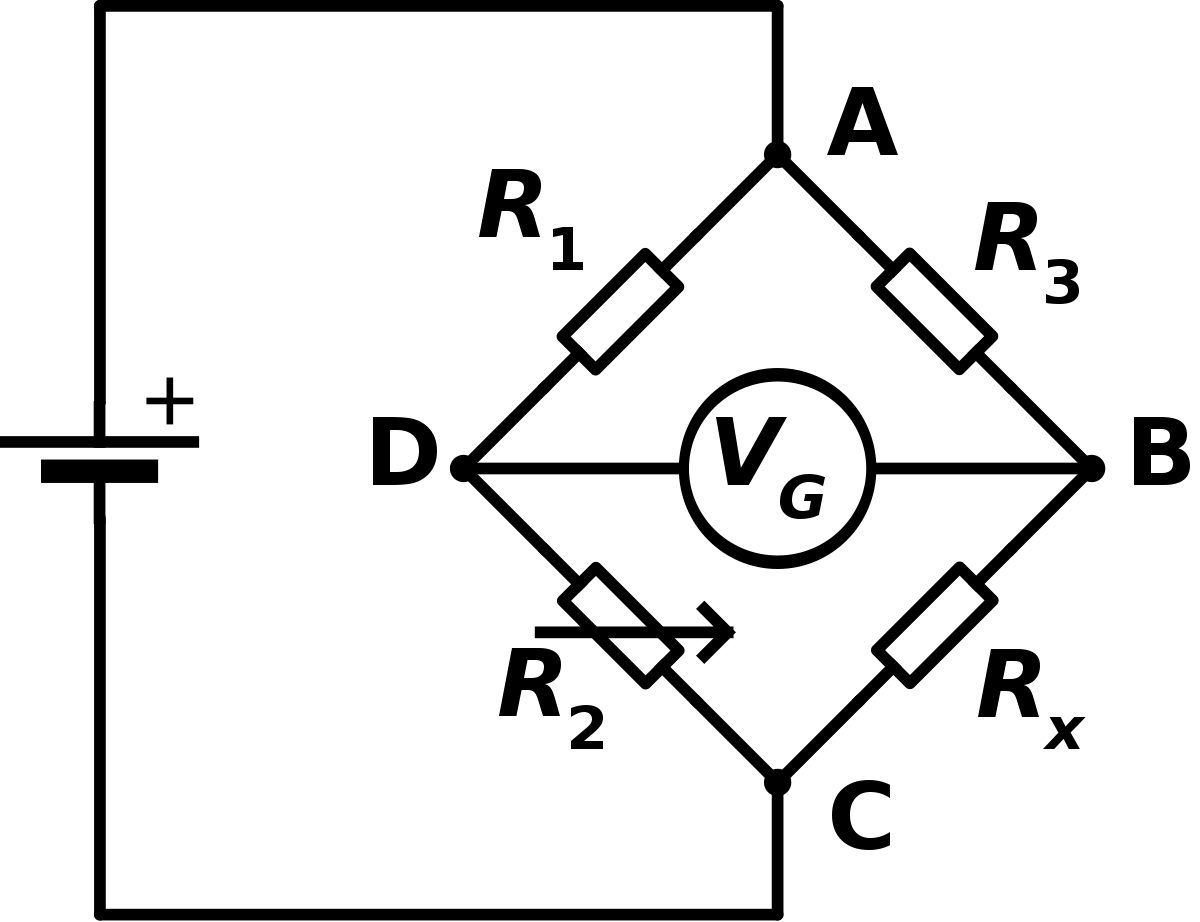
\includegraphics[width=\textwidth]{images/img502.png}
	\end{center}
	\fonte{*internet**}
\end{figure}

Em uma aplicação com sensor de deformação o resistor variável $R_2$ é substituído pela expressão de resistência do extensômetro, e os resistores $R_1$, $R_3$ e $R_x$ são definidos com valores de resistências iguais ao do valor nominal do sensor utilizado, logo, utilizando as leis de Kirchoff para o circuito, a equação de transferência do circuito é mostrada na \autoref{eq:Eq_508}.

\begin{equation}\label{eq:Eq_508}
\frac{V}{V_{in}} = \frac{K \varepsilon}{4 = K \varepsilon}
\end{equation}

onde

Vin: Tensão de alimentação do circuito

V: Tensão mostrada pelo voltímetro Vg


